\documentclass{article}
\usepackage[T1]{fontenc}
\usepackage{lmodern}
\usepackage{graphicx}
\usepackage{amsmath,amssymb}
\usepackage[a4paper,margin=2cm]{geometry}
\usepackage[absolute,overlay]{textpos}
\setlength{\TPHorizModule}{1mm}
\setlength{\TPVertModule}{1mm}
\usepackage[indonesian]{babel}
\usepackage{hyperref}
\setlength{\emergencystretch}{2em}
% unit: Halaman 52

\begin{document}

% === Halaman 52 (llm) ===

\section*{Kriptografi pada Zaman Yunani dan Romawi Kuno}

\begin{itemize}
    \item Di Yunani, kriptografi sudah digunakan 400 BC
    \item Alat yang digunakan: scytale
\end{itemize}

\vspace{40mm}

Plainteks: KILLKINGTOMORROWMIDNIGHT \\
Ciphrteks: KIMWIINOMGLGRIHLTRDTKOON

% deskripsi: Ilustrasi scytale yang memperlihatkan pita kertas tergulung dengan teks terenkripsi 'KILL KING TOMORROW MIDNIGHT'.
% bbox normalisasi: [0.1800, 0.4900, 0.4800, 0.7400]
\begin{textblock*}{63.00mm}(37.80mm,145.53mm)
\noindent
\includegraphics[width=63.00mm,height=74.25mm]{../../images/llm/page_052_img_01.png}%
\end{textblock*}

% deskripsi: Ilustrasi dua prajurit Yunani kuno sedang menggunakan alat scytale untuk berkomunikasi secara rahasia.
% bbox normalisasi: [0.5400, 0.4200, 0.8400, 0.7800]
\begin{textblock*}{63.00mm}(113.40mm,124.74mm)
\noindent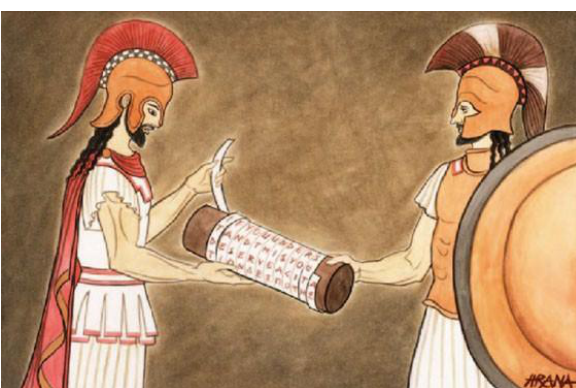
\includegraphics[width=63.00mm,height=106.92mm]{../../images/llm/page_052_img_02.png}%
\end{textblock*}

\end{document}
